\chapter{Correlation Power Analysis} \label{chap:fobos-cpa}

Once acquisition is complete, Correlation Power Analysis (CPA) can be performed.
User must provide their own power model and calculate hypothetical power for each key guess.
FOBOS takes the hypothetical power for each key guess and uses a correlation method e.g. Pearson's coefficient and calculates the correlation values.
The key guess that achieves the highest correlation is a candidate for correct key.

The Analysis module is used to perform DPA attack on power traces collected by the Acquisition
module. To Perform CPA, two inputs are needed, the power traces and and hypothetical power.


\section{FOBOS Data Analysis Module:}
The Data Analysis module consists of 3 sub-modules as shown below:
\begin{itemize}
\item Signal Alignment Module
\item Post processing Module
\item SCA Module
\item Statistics Module
\end{itemize}

\subsection{Post processing Module}
Currently FOBOS supports three Post processing sub modules. They are:
\begin{enumerate}
\item Sample Space Disposition
\item Compression
\item Trace Expunge
\end{enumerate}

\textbf{Space Disposition} allows user to select a part of the trace to perform further post processing
or to perform statistical testing. This also reduces computation time during statistical testing.

\begin{figure}[ht]
\begin{center}
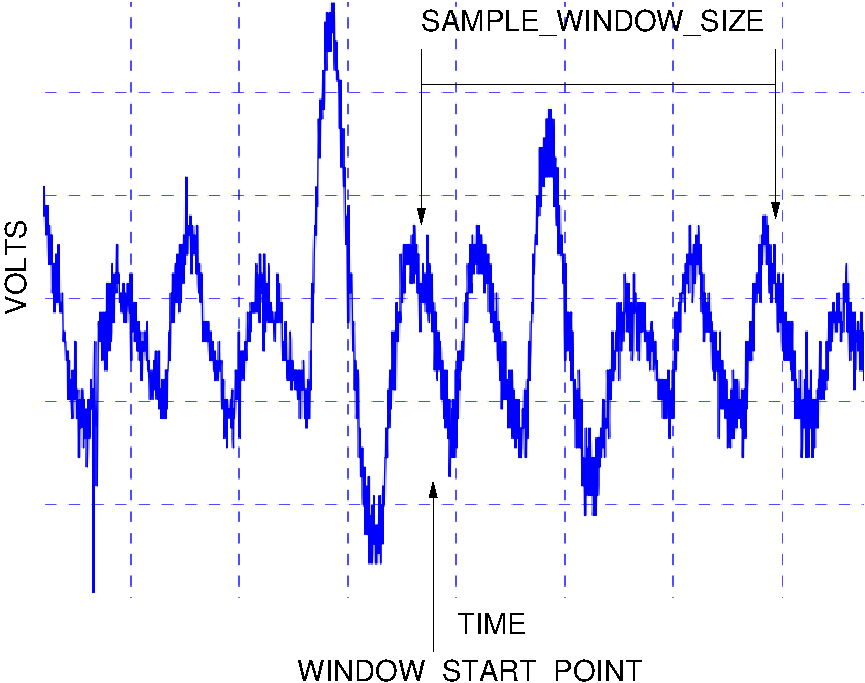
\includegraphics[scale=0.6]{figures/sampleSpaceDisp}
\caption{\label{fig:ssd}Sample Space Disposition}
\end{center} 
\vspace{-3ex}
\end{figure}

The parameters which facilitate this selection are "WINDOW START POINT" and "SAMPLE WINDOW SIZE". As shown in
Fig~\ref{fig:ssd} "WINDOW START POINT" parameter indicate which point in time to further sample the trace and the
"SAMPLE WINDOW SIZE" parameter indicates the number of points to be sampled and stored to a new trace.

\textbf{Compression} allows user compress the power trace in chunks or as a whole
depending upon the user requirement by using the "COMPRESSION LENGTH" parameter as shown in Fig~\ref{fig:cmp}
The user can also the type of compression to be used. They are:
\begin{itemize}
\item Max: Can compress the user specified sample size to the maximum of the given sample set.
\item Min: Can compress the user specified sample size to the minimum of the given sample set.
\item Mean: Can compress the user specified sample size to the average of the given sample set.
\end{itemize}

This also reduces computation time during statistical testing.

\begin{figure}[ht]
\begin{center}
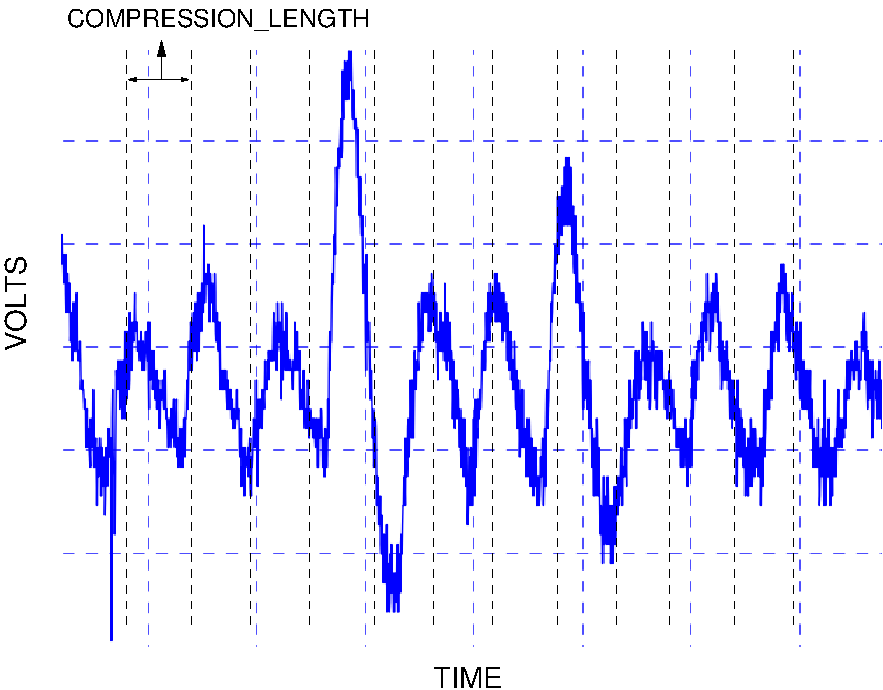
\includegraphics[scale=0.6]{figures/compression}
\caption{\label{fig:cmp}Compression}
\end{center} 
\vspace{-3ex}
\end{figure}

\textbf{Trace Expunge} allows user to selectively "expunge" or discard one or more traces 
depending upon two different selection criteria:

\begin{itemize}
\item Variance: User specifies Upper and Lower bound values. A given trace is removed if its variance (of the entire trace)
is above upper limit or below lower limit.
\item Standard Deviation: User specifies Upper and Lower bound values. A given trace is removed if its standard 
deviation (of the entire trace) is above upper limit or below lower limit.
\end{itemize}

\begin{figure}[ht]
\begin{center}
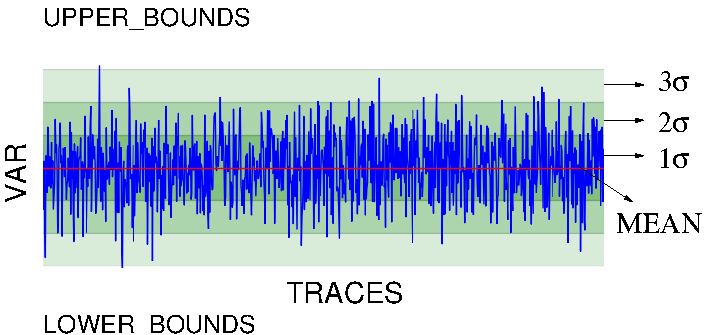
\includegraphics[scale=0.6]{figures/traceExpungMod}
\caption{\label{fig:tex}Trace Expunge}
\end{center} 
\vspace{-3ex}
\end{figure}

This will help in removing traces which are heavily influenced by factors like measurement artefacts etc.

\subsection{SCA Module}
Currently FOBOS supports following Side-channel distinguishers:
\begin{itemize}
\item Pearson's r
\item Spearman's RHO
\end{itemize}
\textbf{Pearson's r}
We assume a linear relationship between the power consumption of the device
and the data being processed. Hence we use Pearson product-moment correlation
coefficient (r), commonly known as Pearson's correlation to correlate instantaneous power
consumption with hamming distance model.

The Pearson's correlation (r) between the the power consumption of the device P and the
hypothetical power model H is given by the Eq.~\ref{eq:pearsons-r}

\begin{equation}\label{eq:pearsons-r}
r(P,H) =\frac{n \sum_{i}^{n}{P_iH_i}-\sum_{i}^{n} P_i\sum_{i}^{n}H_i}{\sqrt{n\sum_{i}^{n} 
	      P_i^2-(\sum_{i}^{n} P_i)^2}\sqrt {n\sum_{i}^{n} H_i^2-(\sum_{i}^{n} H_i)^2}}
\end{equation}   

Correlation Power Analysis (CPA) is a form of DPA where we use a different statistical test to obtain the secret key. Henceforth, we use
the term DPA and CPA alternatively throughout this document.

\textbf{Spearman Rank coefficient}, on the other hand, is a measure of monotonic relationship 
between two variables, in this case between power consumption and power model.
The Rank correlation between power consumption samples P and power consumption hypothesis samples G is given by
\begin{equation}
\label{pceqn}
RHO(P,G)=1-\frac{6\sum_{i}^{n}d_i^2}{n(n^2-1)}
\end{equation} 
where $d_i$ =$P_i$ - $G_i$, and $P_i$, $G_i$ are ranks of the variables P and G 

\subsection{Statistics Module}
FOBOS currently supports following statistic functions.
\begin{itemize}
\item Mean : Calculates mean of the trace, both trace and sample wise, as shown in Fig~\ref{fig:tvs}.
\item Standard Deviation : Calculates Standard Deviation of the trace, both trace and sample wise, as shown in Fig~\ref{fig:tvs}.
\item Variance : Calculates Variance of the trace, both trace and sample wise, as shown in Fig~\ref{fig:tvs}.
\end{itemize}

\begin{figure}[ht]
\begin{center}
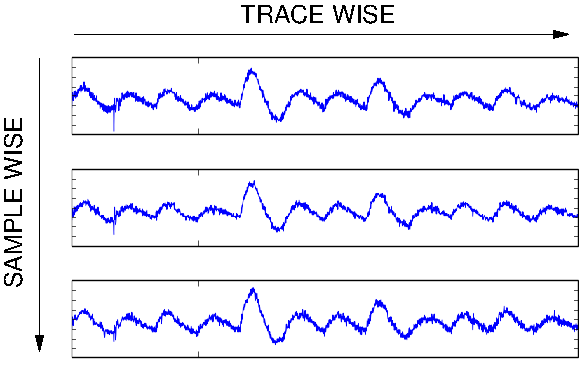
\includegraphics[scale=0.6]{figures/sampleVstrace}
\caption{\label{fig:tvs}Trace wise vs Sample wise}
\end{center} 
\vspace{-3ex}
\end{figure}

\section{Steps to perform CPA using FOBOS}
\subsection{Hypothetical power calculation}
Note: This description uses an example case where key is guessed one byte at a time. \newline
Power model or hypothetical power data is user provided. FOBOS uses a text file for each key
byte. This file includes a line for each key guess value (i.e. 0-255). Each line inculdes hypothetical
power value for the specific key guess for all encryptions. Each value is an integer and separated
from the next value by a space. The text below is an example for one key byte. The first number is the
hypthetical power when the byte equals zero for the frist encryption, first value in the second line is
the estimated power when the key byte equals one for the first encryption and so on.
FOBOS expects to find these files at \texttt{\$fobos/data/}.

Here is sample of the hypothetical power file for byte 0.

\begin{verbatim}
6 4 4 2 5 4 3 5 7 4 5 5 7 3 4 6 5 2 4 5 3 4 3 4 7 4 ….
5 3 4 5 4 2 5 7 4 4 2 4 3 2 4 4 3 4 2 4 3 6 3 2 1 5 ….
.
.
.
\end{verbatim}

\section{CPA configuration}

There are few configuration files that controls the CPA analysis.
Here we list all the configuration parameters used in the FOBOS Analysis and description of their usage.
\subsection{Data Analysis Parameters}

File: \texttt{fobos/config/dataAnalysisParams.txt}
\begin{itemize}
 \item WORK\_DIR \newline
 Directory to save analysis files(Inside the measurements directory). \newline
 Possible Values: file name \newline
 Example: analysis 
 \item MEASUREMENT\_WORK\_DIR \newline
 The name of the measurement directory. \newline
 Possible Values: directory name. \newline
 Example: workspace
 \item TAG \newline
 The type of prefix for the directory name. Used to distinguish different runs. \newline
 Possible Values: counter \newline
 Example: counter
\end{itemize}

\subsection{Sample Space Disposition}

File: samplesSpacesDisp.txt
\begin{itemize}
 \item SAMPLE\_WINDOW\_SIZE \newline
  Number of samples (per trace) to be used in analysis. \newline
  Possible values : Number (e.g. 2000)
 \item SAMPLE\_WINDOW\_START \newline
 The number of the first sample in the window.\newline
 Possible values: Number (e.g. 100)
\end{itemize}

\subsection{Compression Parameters}
File: signalAlignmentParams.txt
\begin{itemize}
 \item COMPRESSION\_LENGTH \newline
 Number of samples to be compressed into one samples. \newline 
 Possible values : Number (e.g. 10)
 \item COMPRESSION\_TYPE \newline 
 The operation to be performed to generate the compressed sample.\newline
 Possible values : MEAN $|$ MAX $|$ MIN
\end{itemize}

\subsection{Sample Analysis Configuration Files}

\begin{verbatim}
dataAnalysisParams.txt 
####################################################
WORK_DIR = FOBOSAnalysis 
MEASUREMENT_WORK_DIR = FOBOSWorkspace 
TAG = counter


compressionParams.txt 
#################################################### 
######## Compression Module Parameters ############# 
#################################################### 
COMPRESSION_LENGTH = 10 
COMPRESSION_TYPE = MEAN # MAX|MIN|MEAN 

sampleSpaceDispParams.txt 
#################################################### 
#### Sample Space Disposition Module Parameters #### 
#################################################### 
SAMPLE_WINDOW_SIZE = 3000 
SAMPLE_WINDOW_START = 3000

\end{verbatim}


\section{Running Data Analysis}

Data Analysis can be run as follows: \newline
\texttt{\$cd \$fobos/bin} \newline
\texttt{\$python dataAnalysis.py} \newline

Once this is done, the script reads the measured and hypothetical power data, runs CPA and
produces several output files. The script prompts the user for the directory that contains the traces
and then uses the power data in the measurements directory as input.  The script
will create a new directory each time it runs. This directory is created in the project directory. Output files will be saved in \texttt{fobos/$<$workspace$>$/$<$projectDir$>$/analysis/}.

\section{CPA Attack on AES using FOBOS}

This section describes a Correlation Power Analysis (CPA) attack of an implementation of the
Advanced Encryption Standard (AES) using FOBOS. 
AES is an symmetric-key cipher used extensively
in security sensitive applications world wide. AES applies four different transformations,
SubBytes, ShiftRows, MixColumns, and AddRoundKey, per round and iterates through several 
such rounds depending upon the key size. An intermediate key called 
"round key" is generated and used per round which is derived from the original key through 
a reversible key scheduling function. We have implemented a basic iterative architecture 
of AES with 128-bit 
key length and 128-bit wide datapath requiring 11 clock cycles for one encryption.
Key scheduling is done on-the-fly and the SubBytes function is realized through look-up-tables.
The block diagram for this design is shown in Fig.~\ref{fig:fobos-aes128}.

\begin{figure}[ht]
\begin{center}
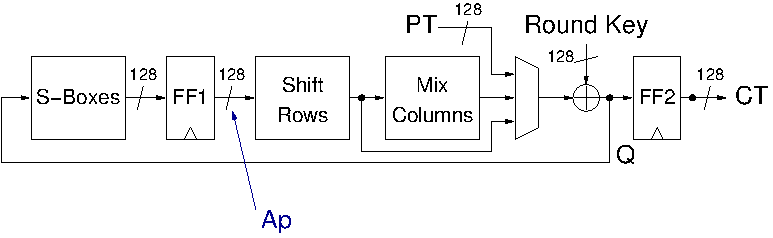
\includegraphics[scale=0.8]{figures/aes128}
\caption{Block Diagram of the AES Core}\label{fig:fobos-aes128}
\end{center} 
\vspace{-3ex}
\end{figure}

We attack our AES design during the first round at the output of the register \textsf{FF1} 
indicated by \textsf{Ap} in Fig.~\ref{fig:fobos-aes128}.
%In order to decrease the loading time of the new plaintext (PT), we reuse the ciphertext (CT)
%as the PT for the next encryption. 
The equation for calculating the Hamming Distance (HD) is shown 
in~\ref{eq:hamm-aes}. We use Pearson's Correlation to correlate the instantaneous
power consumption with the HD model. 

\begin{equation}\label{eq:hamm-aes}%
P_{est.} = \mathrm{HD}(\mathrm{SBOX}(CT_{i}), \mathrm{SBOX}(k_{guess} \oplus PT_{i+1}))
\end{equation}


\begin{figure}[ht]
\begin{center}
\includegraphics[scale=0.8]{figures/victimwrapper}
\caption{\label{fig:fobos-vicaes128}AES Core with Wrapper on Victim FPGA}
\end{center} 
\vspace{-3ex}
\end{figure}

FOBOS Control sends data and key from files, which are in
the format of ASCII coded Hexadecimal values, to the victim. FOBOS Control sets the timeout
to 30,000 clock cycles and the trigger to 4 clock cycles after processing starts.
The victim clock is set to run at 500\,KHz and the result will be 
stored in hexadecimal values in the output file.
% which is located in the corresponding project folder.

The FOBOS control sends the data from the oscilloscope i.e.\ the power traces, inputs, and outputs to
the data analysis module. The first step involves processing the raw 
power trace using the preamble information to obtain the \emph{measured\_power\_trace}.

\begin{figure}[H]
\begin{center}
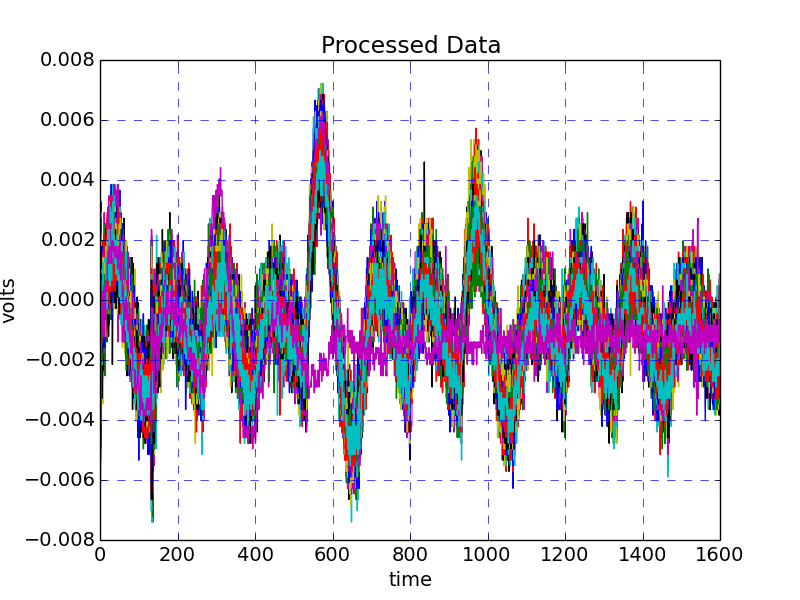
\includegraphics[scale=0.8]{figures/scaTrace1}
\caption{\label{fig:alpt}Aligned Power Trace}
\end{center} 
\vspace{-3ex}
\end{figure}

\begin{figure}[H]
\begin{center}
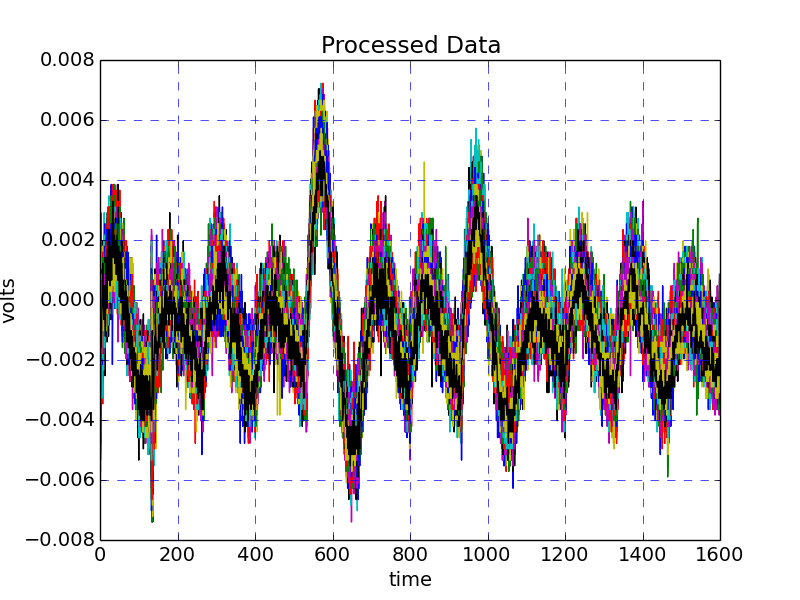
\includegraphics[scale=0.8]{figures/scaTrace2}
\caption{\label{fig:pttx}Power Trace after Trace Expunge}
\end{center} 
\vspace{-3ex}
\end{figure}

We further process the resultant power trace using sample space disposition and compression. The resultant
power traces are shown in Fig.~\ref{fig:ptsp} and Fig.~\ref{fig:ptcp}.

\begin{figure}[H]
\begin{center}
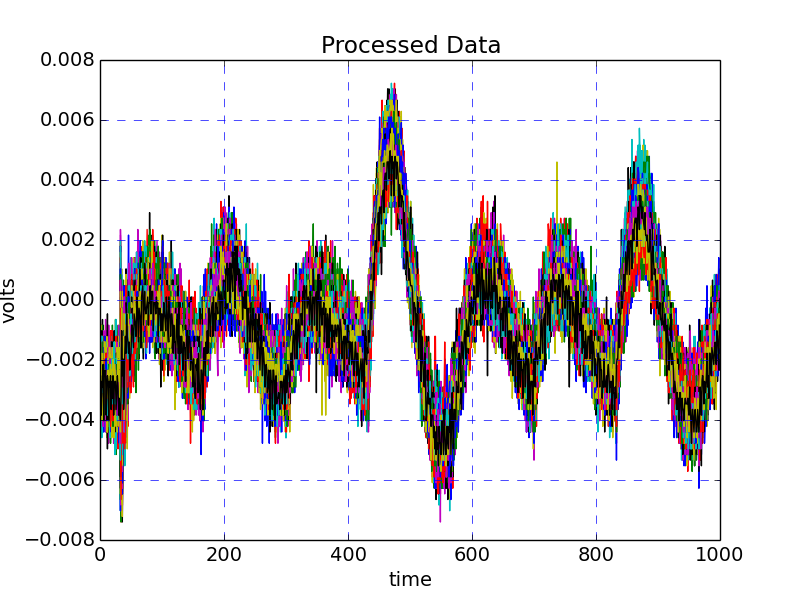
\includegraphics[scale=0.8]{figures/scaTrace3}
\caption{\label{fig:ptsp}Power Trace after Sample Space Disposition}
\end{center} 
\vspace{-3ex}
\end{figure}

\begin{figure}[H]
\begin{center}
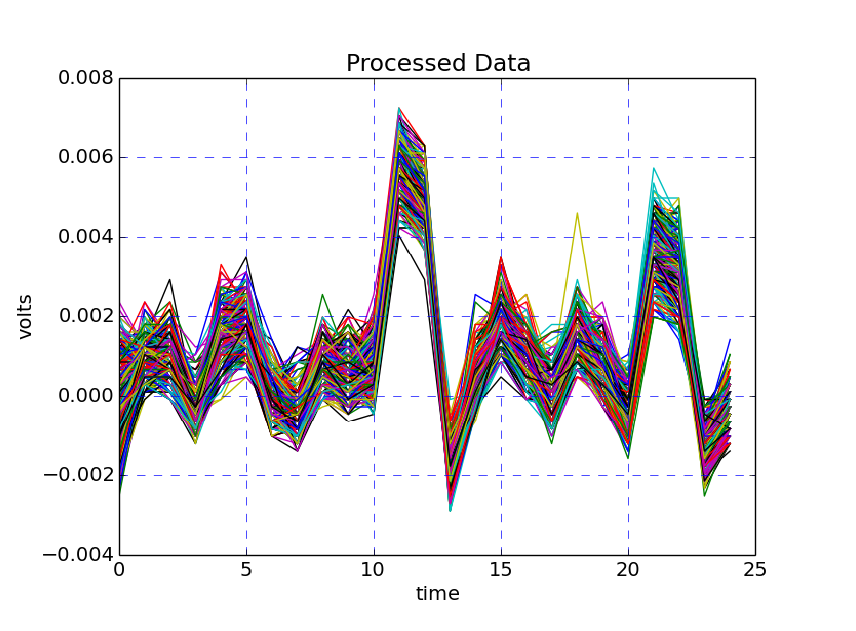
\includegraphics[scale=0.8]{figures/scaTrace4}
\caption{\label{fig:ptcp}Power Trace after Compression}
\end{center} 
\vspace{-3ex}
\end{figure}

The CPA attack is conducted on a sub-byte of the key depending upon the user choice. Hence 
there are 256 different key guess values and correspondingly 9 different HD values i.e.\ 0 $\rightarrow$ 8.
A snippet of the \emph{est\_power\_traces} per key guess value is shown in Fig~\ref{fig:fobos-estpower}. 
\begin{figure}[ht]
\begin{verbatim}
4 6 3 4 5 1 5 4 4 2 4 3 5 6 3 4 4 3 4 2 . . . .
3 2 7 6 5 6 5 5 7 3 5 4 4 2 6 5 2 3 2 5 . . . .
5 4 3 6 4 5 3 4 3 3 6 5 3 0 2 5 6 5 6 5 . . . .
. . . .
\end{verbatim}
\caption{\label{fig:fobos-estpower}Hypothetical Power Model}
\end{figure}

The sca module then calculates the Pearson's Correlation and Spearman's Rank correlation
for all the key guesses by correlating 
the \emph{est\_power\_traces} and \emph{processed\_power\_trace}. 
Snippets of the output logs of the Pearson's and Spearman's Correlation are shown
in Fig.~\ref{fig:pearson} and Fig.~\ref{fig:spearman} respectively.

\begin{figure}[h]
\begin{verbatim}
Window[0] Key Byte- 0x5d [93] Correlation- 0.080
Window[1] Key Byte- 0x9c [156] Correlation- 0.078
Window[2] Key Byte- 0x9c [156] Correlation- 0.086
Window[3] Key Byte- 0x6 [6] Correlation- 0.086
Window[4] Key Byte- 0x16 [22] Correlation- 0.109
Window[5] Key Byte- 0x16 [22] Correlation- 0.175
Window[6] Key Byte- 0xa3 [163] Correlation- 0.087
Window[7] Key Byte- 0xd7 [215] Correlation- 0.082
\end{verbatim}
\caption{\label{fig:pearson}CPA using Pearson's r Log file}
\end{figure}

\begin{figure}[h]
\begin{verbatim}[frame=single]
Window[0] Key Byte- 0x5d [93] Correlation- 0.082
Window[1] Key Byte- 0x9c [156] Correlation- 0.083
Window[2] Key Byte- 0x78 [120] Correlation- 0.109
Window[3] Key Byte- 0x6 [6] Correlation- 0.083
Window[4] Key Byte- 0x16 [22] Correlation- 0.105
Window[5] Key Byte- 0x16 [22] Correlation- 0.176
Window[6] Key Byte- 0xa3 [163] Correlation- 0.086
Window[7] Key Byte- 0xd7 [215] Correlation- 0.091
\end{verbatim}
\caption{\label{fig:spearman}CPA using Spearman's RHO Log file }
\end{figure}

The sca module also plots two graphs, called the Correlation Plot 
shown in Fig.~\ref{fig:prcorrplt} for Pearson's r and Fig.~\ref{fig:spcorrplt} for 
Spearman's RHO respectively.  
The correlation plot shows how well each individual key guess correlates with the power trace.
The peak value of this plot indicates the correct sub-key byte. 

\begin{figure}[H]
\begin{center}
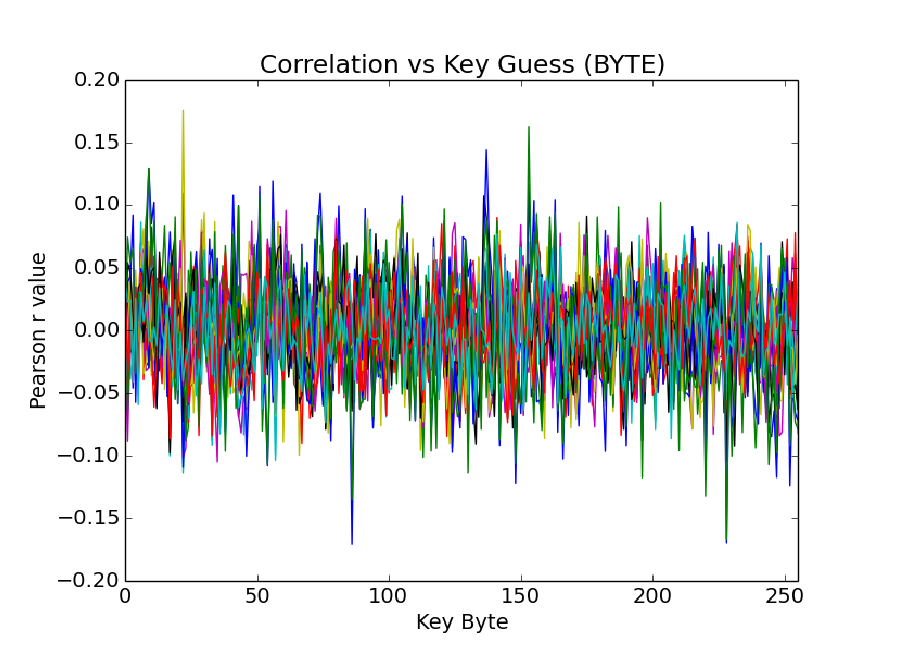
\includegraphics[scale=0.8]{figures/pearson-r}
\caption{\label{fig:prcorrplt}Results of Pearson's r}
\end{center} 
\vspace{-3ex}
\end{figure}

\begin{figure}[H]
\begin{center}
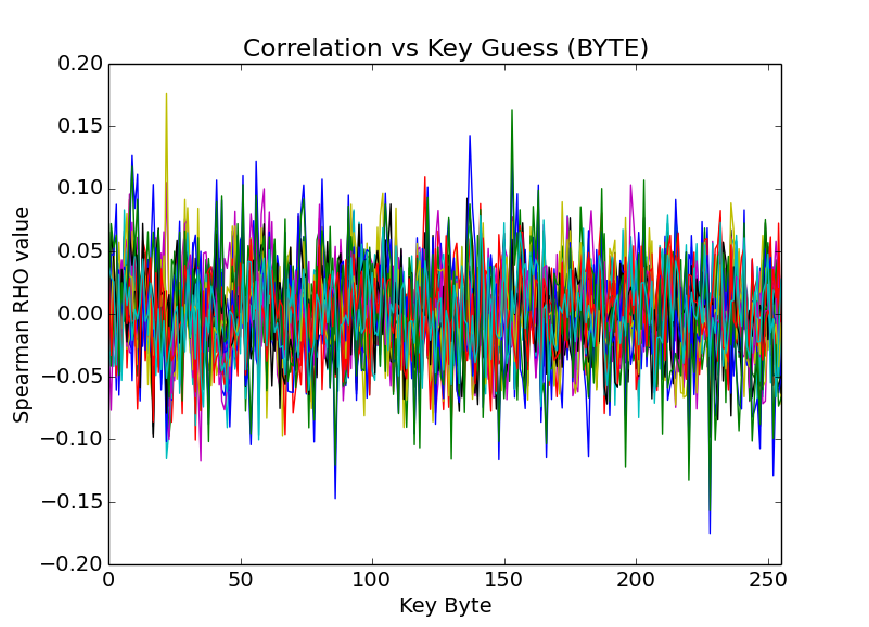
\includegraphics[scale=0.8]{figures/spearman-rho}
\caption{\label{fig:spcorrplt}{Results of Spearman's RHO}}
\end{center} 
\vspace{-3ex}
\end{figure}


